\documentclass{beamer}
\usepackage{HECbeamer}
% \usepackage{pgfpages}
% \pgfpagesuselayout{4 on 1}[letterpaper, landscape, border shrink=5mm]
\title[\color{white}{MATH 60604 \S~7d - Modèle à risques proportionnels de Cox}]{\texorpdfstring{MATH 60604 \\Modélisation statistique \\ \S~7d - Modèle à risques proportionnels de Cox}{MATH 60604 \\ Modélisation statistique \\ \S~7d - Modèle à risques proportionnels de Cox}}
\author{Léo Belzile}
\institute{HEC Montréal\\
Département de sciences de la décision}
\date{} 

\begin{document}
\frame{\titlepage}
% \begin{frame}
%  
% \end{frame}

\begin{frame}
\frametitle{Motivation}
\begin{itemize}
\item L'estimateur de Kaplan--Meier permet d'estimer de manière nonparamétrique la fonction de survie.
\item Qu'est-ce qu'on ferait si on voulait mesurer l'effet de variables explicatives $\mathrm{X}_1, \ldots, \mathrm{X}_p$ sur la survie?
\begin{itemize} 
\item avec des variables catégorielles (et beaucoup de données), on pourra estimer la fonction pour chaque sous-groupe à l'aide de l'estimateur de Kaplan--Meier.
\item cette approche ne fonctionne pas si $\mathrm{X}_j$ est continue ou le nombre d'observations par groupe est petite.
\end{itemize}
\end{itemize}
\end{frame}
% 
% \begin{frame}
% \frametitle{Modèle à risques proportionnels de Cox}
% \begin{itemize}
% \item Le modèle de Cox à risques proportionnels est un modèle \alert{semi-paramétrique} pour la fonction de risque $h(t)$. 
% \begin{itemize}
% \vp \vp
% \item C'est un modèle semi-paramétrique car il comprend à la fois une partie paramétrique et une partie non-paramétrique.
% \item La partie paramétrique du modèle est paramétrisée en terme de coefficients de régression $\beta_1, \ldots, \beta_p$, qui mesure les effets des variables explicatives sur la survie. 
% \end{itemize}
% \end{itemize}
% \end{frame}

\begin{frame}
\frametitle{Fonction de risque cumulative}

Pour $T$ continue${}^*$, la fonction de risque cumulative est
\begin{align*}
H(t) = \int_{0}^{t} h(u) \d u = \int_0^t \frac{f(u)}{1-F(u)}\d u = -\ln\{S(t)\}
\end{align*}
et donc on peut écrire la fonction de survie  
\begin{align*}
S(t) = \exp\{-H(t)\}.
\end{align*}


On peut aussi écrire la log-vraisemblance en terme de la fonction de risque (cumulative)
\begin{align*}
\ell(\bs{\theta}) = \sum_{i=1}^n \{\delta_i \ln h(t_i; \bs{\theta}) - H(t_i; \bs{\theta})\}
\end{align*}
\end{frame}


% \begin{frame}
% \frametitle{Fonction de risque}
% \begin{itemize}
% \item Pour un temps de survie $T$, la \alert{fonction de survie} est $S(t) = \P{T>t}$
% \item[] et la \alert{fonction de répartition} est $F(t) = \P{T\leq t}$
% 
% \item Rappel: on peut écrire la fonction de survie en terme de la fonction de répartition:
% \begin{align*}
% S(t) = 1 - F(t)
% \end{align*}
% \item La \alert{fonction de risque} (ou \alert{taux de défaillance} ou \alert{taux de risque}) est définie comme 
% \begin{align*}
% h(t) = \lim_{\delta \to 0} \frac{\P{t < T<t + \delta \mid T>t}}{\delta} = \lim_{\delta \to 0} \frac{1}{\delta}\frac{\P{t<T<t + \delta}}{\P{T>t}}
% \end{align*}
% \item On peut interpréter la fonction de risque comme étant la probabilité instantanée de ``mourir'' au temps $t$, compte tenu de la survie jusqu'au temps $t$.
% %\item \emph{We can think of the hazard rate as being the instantaneous probability of ``dying'' at temps $t$, given survival to temps $t$. }
% \end{itemize}
% \end{frame}

% \begin{frame}
% \frametitle{Fonction de risque}
% \begin{itemize}
% \item Quand $T$ est continue, on peut montrer que la fonction de risque est en fait
% \begin{align*}
% h(t) = \frac{-\d \ln S(t) }{\d t}
% \end{align*}
% \item On peut donc écrire la \alert{fonction de survie} en terme de la \alert{fonction de risque}:
% \begin{align*}
% S(t) = \exp\left\{ - \int_0^t h(u) \d u \right\}
% \end{align*}
% \item Alors, si on connait la fonction de survie, on peut établir la fonction de risque, et vice versa. 
% \item Connexion entre la courbe de survie et la fonction de risque:
% \begin{itemize}
% \vp \vp
% \item un taux de risque plus faible à $t$ implique une probabilité plus faible que l'événement (ex. la mort) survienne; la courbe de survie a une pente moins prononcée à $t$
% \item un taux de risque plus élevé implique une plus grande probabilité que l'événement (ex. la mort) survienne; la pente de la courbe de survie est plus abrupte à $t$.
% \end{itemize}
% \end{itemize}
% \end{frame}

\begin{frame}
\frametitle{Postulat de risques proportionnels}
Dans le modèle à risques proportionnels, la fonction de risque est
\begin{align*}
 h(t; \mathbf{x}_i) = h_0(t)\exp(\mathbf{x}_i\bs{\beta})
\end{align*}
où
\bi \item la fonction de risque de base, $h_0(t)$ est le seul terme de droite qui varie dans le temps.
\item l'hypothèse dite de \alert{risques proportionnels} est que le rapport $h(t; \bs{x}_i)/h(t; \bs{x}_j)$ est constant peut importe la valeur de $t$.
\item l'interprétation des effets des variables explicatives est simplifiée, parce que ces effets ne varient pas avec le temps.
\item ce postulat est très restrictif et doit être validé en pratique, mais il est particulièrement commode pour les dérivations.
\ei

\textbf{Note:} il n'y a pas d'ordonnée à l'origine dans le modèle de Cox: cette dernière est incorporée dans $h_0(t)$.
% Avec l'hypothèse de risque proportionnels, la fonction de survie devient
% \[
% S(t; \mathbf{x}_i) = \exp\left\{H_0(t_j)\right\}^{\exp(\mathbf{x}_i\bs{\beta})}
% \] 
% et la fonction de densité 
% \begin{align*}
% f(t; \mathbf{x}_i) = \exp(\bs{\beta}\mathbf{x}_i) h_0(t) S_0(t)^{\exp(\bs{\beta}\mathbf{x}_i)}. 
% \end{align*}
\end{frame}
\begin{frame}
 \frametitle{Dérivation du modèle à risques proportionnels}
 
On considère les temps de défaillance observés $0 \leq t_1 < \cdots < t_D$, supposés uniques (pas de doublons) pour simplifier la dérivation.


La fonction de risque cumulative de base,
\[
H_0(t) = \sum_{j: t_j \leq t} h_0(t_j),
\] est une fonction escalier avec des sauts uniquement aux temps de défaillance observés.

On considère 
\bi 
\item $\mathcal{R}_j$, l'ensemble des individus à risques au temps $t_j$
\item $\delta_i$, un indicateur binaire qui vaut $1$ en cas de défaillance observée, et $0$ si l'observation est censurée à droite.
\ei

\end{frame}
\begin{frame}
 \frametitle{Fonction de vraisemblance du modèle de Cox}
 Soit $h_j = h_0(t_j)$ et $g_i=\exp(\mathbf{x}_i \bs{\beta})$. La vraisemblance est
 \begin{align*}
  \ell(\bs{h}, \bs{\beta}) &= \sum_{i=1}^n \left\{ \delta_i \ln (g_ih_i)-g_iH_0(t_j)\right\} 
  \\& =  \sum_{i=1}^n \left\{ \delta_i \ln g_i + \delta_i \ln h_i -h_i \sum_{j \in \mathcal{R}_i}g_j\right\} 
 \end{align*}
Puisqu'on s'intéresse principalement aux effets des variables explicatives $\mathbf{X}$, on considère les paramètres $h_1,\ldots, h_D$ comme des paramètres de nuisance.

Si $\bs{\beta}$ est fixe, le maximum de vraisemblance de $h_i$ est $\widehat{h}_i = \delta_i/\sum_{j \in \mathcal{R}_i} g_j$.
Ce estimé est positif seulement si $\delta_i=1$ (temps de défaillance observé).
\end{frame}
\begin{frame}
 \frametitle{Vraisemblance profilée du modèle de Cox}
 On peut ainsi dériver la log vraisemblance profilée pour $\bs{\beta}$, à savoir
 \begin{align*}
  \ell_{\mathrm{p}}(\bs{\beta}) = \max_{\bs{h}}  \ell(\bs{h}, \bs{\beta})  = \sum_{i=1}^n \delta_i \ln \left( \frac{\exp(\mathrm{x}_i\bs{\beta})}{\sum_{j \in \mathcal{R}_i}\exp(\mathrm{x}_j\bs{\beta})}\right)
 \end{align*}
 Il suffit alors de maximiser $\ell_{\mathrm{p}}(\bs{\beta})$. 
Même si ce modèle a un nombre de paramètres qui excède le nombre d'observations (!), $\ell_{\mathrm{p}}(\bs{\beta})$ se comporte à toute fin pratique comme une vraisemblance ordinaire. 
 \bi \item Erreurs-type via l'information observée.
 \item Tests de rapport de vraisemblance, du score ou de Wald pour les paramètres $\bs{\beta}$.
 \ei 
 \vp\vp
 
 {\footnotesize 
La situation est plus complexe s'il y a des doublons, mais les ajustements sont faits automatiquement par les logiciels (plusieurs options disponibles, certaines meilleurs et plus coûteuses que d'autres).


}
\end{frame}

\begin{frame}
 Une fois les estimés du maximum de vraisemblance $\widehat{\bs{\beta}}$ recouvrés, on peut obtenir la fonction de risque cumulative et la fonction de survie de base
 \begin{align*}
  \widehat{H}_0(t) &= \sum_{i: t_i \leq t} \frac{\delta_i}{\sum_{j \in \mathcal{R}_i} \exp(\mathrm{x}_j\widehat{\bs{\beta}})},
  \intertext{d'où l'estimé de la fonction de survie pour un individu avec covariables $\mathbf{x}$}
  \widehat{S}(t; \mathbf{x}) &= \exp\left\{-\exp(\mathbf{x}\widehat{\bs{\beta}})\widehat{H}_0(t)\right\}
 \end{align*}
\end{frame}


% \begin{frame}
% 
% \begin{itemize}
% \item Le modèle de Cox à risques proportionnels spécifie la fonction de risque comme étant une fonction des variables explicatives. 
% \item Pour un sujet $i$ avec des variables explicatives $\mathrm{X}_{i1}, \ldots, \mathrm{X}_{ip}$, la fonction de risque $h_i(t)$ est écrit comme
% \begin{align*}
% h_i(t) = h_0(t) \exp(\beta_1 \mathrm{X}_{i1} + \cdots + \beta_p \mathrm{X}_{ip})
% \end{align*}
% \item Dans ce modèle, $h_0(t)$ est la fonction de risque de base (``baseline hazards'').
% \begin{itemize}
% \vp \vp
% \item Il s'agit du taux de risque quand toutes les variables explicatives sont $0$.
% \item Notez qu'il n'y a pas de paramètre $\beta_0$ pour l'ordonnée à l'origine --- cette dernière est absorbée dans la fonction de risque de base $h_0(t)$. 
% \item Le modèle de Cox à risques proportionnels n'estemps pas le risque de base $h_0(t)$, il est simplement inclus dans le modèle implicitement\ldots
% \end{itemize}
% \item Remarquez que la partie régression du modèle, $\beta_1\mathrm{X}_{i1} + \cdots + \beta_p \mathrm{X}_{ip}$, ne dépend pas sur le temps $t$! Seul le risque de base $h_0(t)$ dépend sur le temps $t$. 
% \end{itemize}
% \end{frame}
% 
% \begin{frame}
% \frametitle{Modèle de Cox à risques proportionnels}
% \begin{align*}
% h_i(t) = h_0(t) \exp(\beta_1 \mathrm{X}_{i1} + \cdots + \beta_p \mathrm{X}_{ip})
% \end{align*}
% \begin{itemize}
% \item Pour les modèles de régression on est principalement intéressé à mesurer les effets des variables $\mathrm{X}_1, \ldots, \mathrm{X}_p$ sur la variable réponse $T$.
% \item Dans le cadre du modèle de Cox à risques proportionnels, ça veut dire qu'on n'est pas vraiment intéressé par le risque de base $h_0(t)$, et on est plutôt intéressé à la partie régression $\exp(\beta_1 \mathrm{X}_1 + \cdots + \beta_p \mathrm{X}_p)$. 
% \item Le fait que la partie régression du modèle ne dépend pas sur le temps $t$ permet pour une interprétation simplifiée des effets des variables explicatives, parce que ces effets ne varient pas avec le temps!
% \item Comme on a vu plus tôt, il y a une relation entre la fonction de risque et la fonction de survie. Alors, le modèle de Cox à risques proportionnels permet de mesurer les effets des variables explicatives sur la fonction de risque et aussi sur la fonction de survie.  
% \end{itemize}
% \end{frame}

\begin{frame}
\frametitle{Interprétations des paramètres}
\begin{itemize}
\item Pour interpréter les paramètres du modèle de Cox à risques proportionnels, on peut comparer les taux de risques (modèle multiplicatif). 
\item Prenons deux individus qui sont presque identiques, sauf que leurs valeurs pour la variable $\mathrm{X}_j$ diffère par une unité. 
\begin{itemize}
\vp \vp
\item Pour l'individu $i$ avec $\mathrm{X}_{ij}=\mathrm{x}_j+1$, la fonction de risque est
\begin{align*}
h(t; \mathbf{x}_i) = h_0(t) \exp(\beta_0 + \beta_1 \mathrm{x}_1 + \cdots + \beta_j (\mathrm{x}_j+1)+\cdots + \beta_p \mathrm{x}_p)
\end{align*}
\item Pour l'individu $k$ avec $\mathrm{X}_{kj}=\mathrm{x}_j+1$, la fonction de risque est
\begin{align*}
h(t; \mathbf{x}_k) = h_0(t) \exp(\beta_0 + \beta_1 \mathrm{x}_1 + \cdots + \beta_j \mathrm{x}_j+\cdots + \beta_p \mathrm{x}_p)
\end{align*}
\end{itemize}
\item Le \alert{rapport} des fonctions de risque  est
\begin{align*}
\frac{h(t; \mathbf{x}_k)}{h(t; \mathbf{x}_i)} &= 
% \frac{h_0(t) \exp(\beta_0 + \beta_1 \mathrm{x}_1 + \ldots + \beta_j (\mathrm{x}_j+1)+\ldots + \beta_p \mathrm{x}_p)}{h_0(t) \exp(\beta_0 + \beta_1 \mathrm{x}_1 + \ldots + \beta_j \mathrm{x}_j+\ldots + \beta_p \mathrm{x}_p)} \\
% &= \frac{\exp(\beta_j(\mathrm{x}_j+1)}{\exp(\beta_j \mathrm{x}_j)} \\ &=
 \exp(\beta_j)
\end{align*}
\end{itemize}
\end{frame}

\begin{frame}
\frametitle{Rapport de risque}
\begin{itemize}
\item Pour chaque augmentation d'une unité pour la variable $\mathrm{X}_j$, la fonction de risque sera \alert{multipliée} par un facteur $\exp(\beta_j)$, \textit{ceteris paribus}.
\item La quantité $\exp(\beta_j)$ est appelée le \alert{rapport de risques}.
% (``hazard ratio'' ou HR), car elle représente le rapport des taux de risques. 
\begin{itemize}
\vp \vp
\item Si $\exp(\beta_j)=1$,  $\mathrm{X}_j$ n'a pas d'effet sur la fonction de risque.
\item Si $\exp(\beta_j)>1$, le taux de risque \textbf{augmente} quand $\mathrm{X}_j$ augmente. 
\begin{itemize}
\vp \vp
\item Des valeurs plus élevées de $\mathrm{X}_j$ correspondent à un risque plus élevé que l'événement survienne, et donc un temps de survie plus court.
\end{itemize}
\item Si $\exp(\beta_j)<1$, le taux de risque \textbf{diminue} quand $\mathrm{X}_j$ augmente. 
\begin{itemize}
\vp \vp
\item Des valeurs plus élevées de $\mathrm{X}_j$ correspondent à un risque moins élevé que l'événement survienne, et donc un temps de survie plus long.
\end{itemize}
\end{itemize}
\end{itemize}
\end{frame}


% \begin{frame}
% \frametitle{Interprétations des paramètres}
% \begin{itemize}
% \item Alors, pour chaque augmentation d'une unité pour la variable $\mathrm{X}_j$, la fonction de risque sera \alert{multipliée} par un facteur de $\exp(\beta_j)$, lorsque \alert{toutes les autres variables restent inchangées.}
% \item La quantité $\exp(\beta_j)$ est appelée le \alert{ratio de risque} (``hazard ratio'' ou HR), car elle représente le rapport des taux de risques. 
% \begin{itemize}
% \vp \vp
% \item Si $\exp(\beta_j)=HR=1$, ça veut dire que le ratio ${h_i(t)}/{h_k(t)}=1$, et donc  $\mathrm{X}_j$ n'a pas d'effet sur la fonction de risque.
% \item Si $\exp(\beta_j)=HR>1$, le ratio ${h_i(t)}/{h_k(t)}>1$, et donc le taux de risque \alert{augmente} quand $\mathrm{X}_j$ augmente. 
% \begin{itemize}
% \vp \vp
% \item Cela signifie que des valeurs plus élevées de $\mathrm{X}_j$ correspondent à un risque plus élevé que l'événement survienne, et donc des prévisions de temps de survie plus courts.
% \end{itemize}
% \item Si $\exp(\beta_j)=HR<1$, le ratio ${h_i(t)}/{h_k(t)}<1$, et donc le taux de risque \alert{diminue} quand $\mathrm{X}_j$ augmente. 
% \begin{itemize}
% \vp \vp
% \item Cela signifie que des valeurs plus élevées de $\mathrm{X}_j$ correspondent à un risque moins élevé que l'événement survienne, et donc des prévisions de temps de survie plus longs.
% \end{itemize}
% \end{itemize}
% \end{itemize}
% \end{frame}

\begin{frame}
\frametitle{Exemple avec données \code{melanome}}
Le fichier \texttt{melanome} contient des données de survie pour des patients atteints d'une tumeur maligne, un mélanome qui a été enlevé lors d'une opération chirurgicale. La base de données contient les variables suivantes:


{ \footnotesize
\begin{itemize}
\item \code{temps}: temps de survie (en jours) depuis l'opération 
\item \code{statut}: \code{1} si le patient est mort, \code{0} si le temps est censuré
\item \code{sexe}: sexe du patient, soit \code{1} pour les hommes et \code{0} pour les femmes
\item \code{age}: l'âge (an années) au moment de l'opération
\item \code{annee}: l'année de l'opération
\item \code{epaisseur}: l'épaisseur (en mm) de la tumeur
\item \code{ulcere}: variable indicatrice, \code{1} en cas d'ulcération, \code{0} sinon.
\end{itemize}
}

\end{frame}

\begin{frame}
\frametitle{Statistiques descriptives pour données \code{melanome}}
\begin{center}
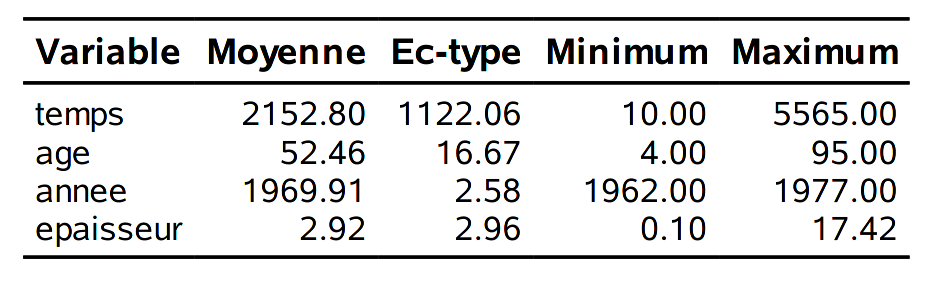
\includegraphics[width = 0.5\textwidth]{img/c7/diapos7e10}
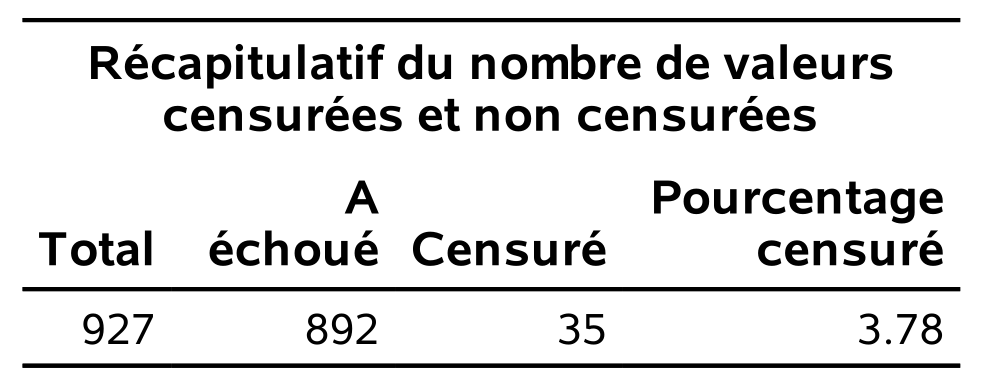
\includegraphics[width = 0.5\textwidth]{img/c7/diapos7e09}
\end{center}
\end{frame}

\begin{frame}[fragile]
\frametitle{Modèle de Cox pour données \code{melanome}}
 Le modèle de Cox à risques proportionnels est 
\begin{align*}
h(t) = h_0(t) \exp( \beta_1 \code{sexe} + \beta_2 \code{age} + \beta_3 \code{epaisseur} + \beta_4 \code{ulcere})
\end{align*}
 On peut ajuster ce modèle dans \SASlang{} avec la procédure \code{phreg}:
\vp \vp
\begin{tcolorbox}[colback=white,colframe=hecblue,title=Code \SASlang{} pour le modèle à risque proportionnel]
{\footnotesize 
\begin{verbatim}
prod phreg data=modstat.melanome;
model temps*statut(0) = sexe age epaisseur ulcere / ties=exact;
run;
\end{verbatim}
}
\end{tcolorbox}
\end{frame}

\begin{frame}
\frametitle{Tests basés sur la vraisemblance}
\vp \vp
\begin{center}
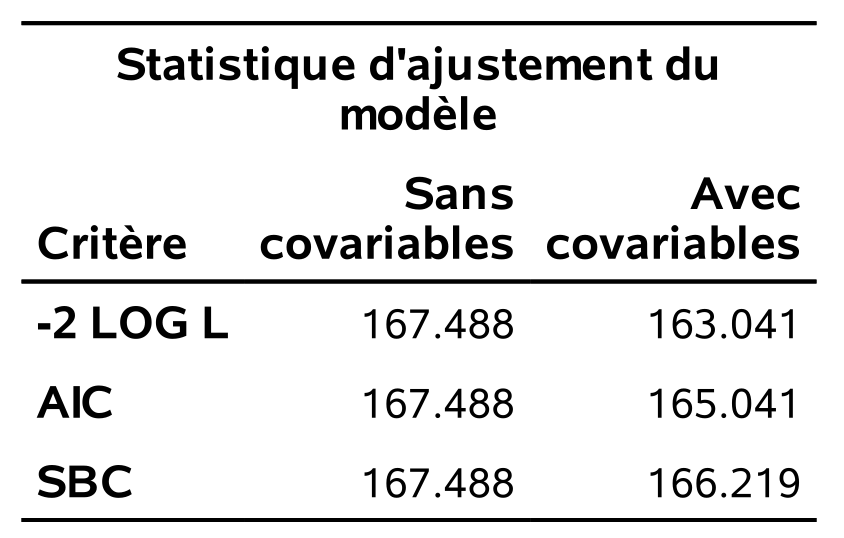
\includegraphics[width = 0.5\textwidth]{img/c7/diapos7e12}
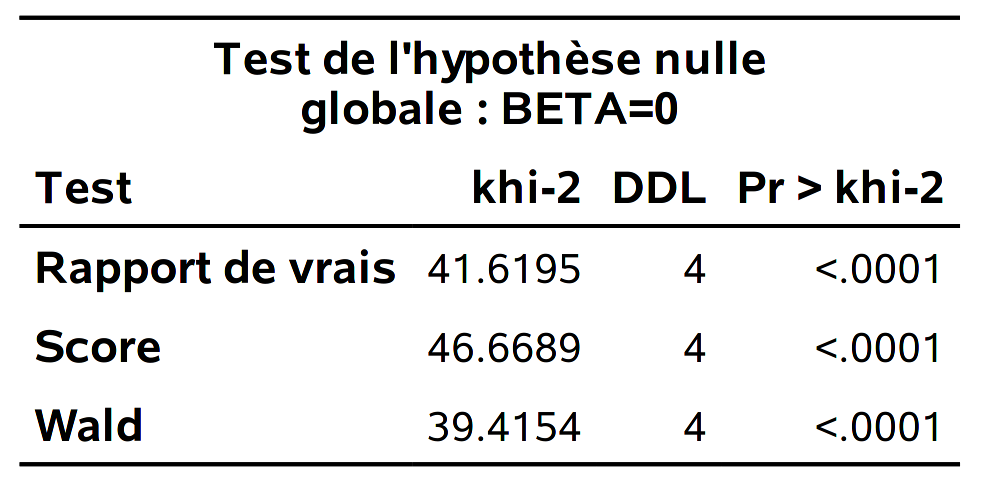
\includegraphics[width = 0.5\textwidth]{img/c7/diapos7e13}
\end{center}
{\footnotesize
La sortie inclut la valeur de la log-vraisemblance avec et sans variables explicatives, et les tests usuels pour $\Hy_0: \bs{\beta}=\bs{0}_p$ versus $\Hy_a: \bs{\beta} \neq \bs{0}_p$.

}
\end{frame}

\begin{frame}
\frametitle{Coefficients estimés du modèle de Cox}
\vp \vp
\begin{center}
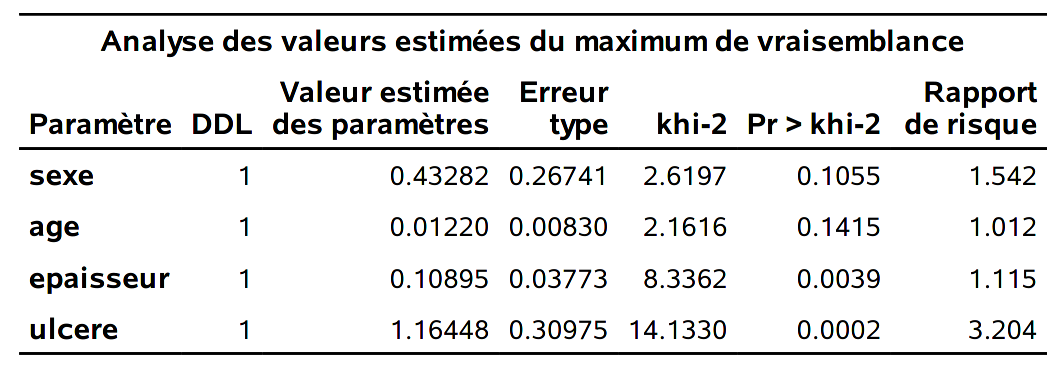
\includegraphics[width = 0.8\textwidth]{img/c7/diapos7e14}
\end{center}
% 

\end{frame}

\begin{frame}
\frametitle{Interprétation}
\begin{itemize}
\item Pour la variable \code{sexe}, $\exp(\widehat{\beta}_1)=1.542$ représente le rapport de risque entre un homme et une femme du même âge, avec la même épaisseur de tumeur et le même état d'ulcération. Ainsi, le taux de risque pour les hommes est $1.542$ fois celui pour les femmes, lorsque toutes les autres variables restent inchangées.
\item Pour la variable \code{epaisseur}, $\exp(\widehat{\beta}_3)=1.115$. Pour chaque augmentation de 1mm de l'épaisseur de la tumeur, le taux de risque augmente d'un facteur de $1.115$ (ou 11.5\%), lorsque toutes les autres variables restent inchangées. 
\end{itemize}
\end{frame}
% 
% 
% \begin{frame}
% \frametitle{Exemple}
% \textbf{Sortie SAS:}
% \vp \vp
% \begin{center}
% \includegraphics[scale=0.7]{img/c7/mel_cph_2.png}
% \end{center}
% \begin{itemize}
% \item On voit qu'il y a de différents tests pour
% \begin{itemize}
% \vp \vp
% \item[] $\Hy_0: \beta_1 = \cdots = \beta_4 = 0 $
% \item[] $\Hy_1$ au moins un $\beta_j$ est différent de zéro.
% \end{itemize}
% \end{itemize}
% \end{frame}
% 
% \begin{frame}
% \frametitle{Quelques remarques\ldots}
% \begin{align*}
% h_i(t) = h_0(t) \exp(\beta_1 \mathrm{X}_{i1} + \cdots + \beta_p \mathrm{X}_{ip})
% \end{align*}
% \begin{itemize}
% \item Dans le modèle de Cox à risques proportionnels, l'hypothèse sous-jacente est que les effets des variables explicatives sont \alert{constants à travers le temps}. C'est la condition de \alert{risques proportionnels}.
% \begin{itemize}
% \vp \vp
% \item On suppose que l'effet de la variable $\mathrm{X}_j$ sur la fonction de risque $h(t)$ est toujours $\exp(\beta_j)$, peut importe le temps $t$. 
% \item Il y a certainement des situations dans lesquelles cette condition ne sera pas valide. Ex: pour des ages $<18$, les hommes on un taux de risque moins élevé que les femmes, mais pour les ages $\geq 18$, le taux de risque pour les hommes est plus élevés que ceux des femmes.
% \item On peut tester formellement si cette condition est satisfaite, mais on ne verra pas cela.
% \end{itemize}
% \end{itemize}
% \end{frame}

% \begin{frame}
% \frametitle{Quelques remarques\ldots}
% \begin{align*}
% h_i(t) = h_0(t) \exp(\beta_1 \mathrm{X}_{i1} + \cdots + \beta_p \mathrm{X}_{ip})
% \end{align*}
% \begin{itemize}
% \item Dans le modèle de Cox à risques proportionnels, on ne modélise pas la fonction de risque de base $h_0(t)$. 
% \item Rappel: il y a une relation entre la fonction de survie et le taux de risque:
% \begin{align*}
% S(t) = \exp \left\{-\int_0^t h(u) du \right\}
% \end{align*}
% \item Dans le cadre du modèle de Cox à risques proportionnels, on obtient
% \begin{align*}
% S(t) = \exp \left\{-\exp(\beta_1 \mathrm{X}_1 + \cdots + \beta_p \mathrm{X}_p) \int_0^t h_0(u) du \right\}
% \end{align*}
% \item Alors, si on veut estimer la fonction de survie en terme des variables explicatives $\mathrm{X}_1, \ldots, \mathrm{X}_p$, il faudra modéliser la fonction de risque de base $h_0(t)$. 
% \begin{itemize}
% \vp \vp
% \item Il y a plusieurs façons de modéliser $h_0(t)$. On peut le faire de façon non-paramétrique (ex: l'estimateur Kaplan--Meier)\ldots 
% \end{itemize}
% \end{itemize}
% \end{frame}
% 
% \begin{frame}
% \frametitle{Quelques remarques\ldots}
% \begin{itemize}
% \item Il y a plusieurs différents modèles, autres que le modèle de Cox à risques proportionnels, qu'on peut utiliser dans le cadre d'analyse de survie. 
% \item L'analyse de survie est particulièrement difficile, et la présence de la censure rend l'estimation encore plus difficile. 
% \end{itemize}
% \end{frame}




\end{document}
